\chapter{Logiikka ja matematiikka}

Matematiikka on logiikan keskeinen sovellusalue. Matematiikan rakenteita tutkivaa logiikan aluetta kutsutaan matemaattiseksi logiikaksi. Matemaattisessa logiikassa tutkitaan lauseita, joissa loogisten symbolien lisäksi voi esiintyä matemaattisia merkintöjä, kuten yhtäsuuruus, lukuja, muuttujia tai laskutoimituksia. Matemaattisen logiikan tutkimuskohteita ovat matemaattiset teoriat ja todistukset.


% (pelkästään matematiikkaa sivuavia esimerkkejä)
\section{Joukko-oppia}% (mahdollisesti lisämateriaalia)}
Seuraavaksi tutkitaan logiikan soveltamista matemaattisiin rakenteisiin, joita kutsutaan \termi{joukko}{joukoiksi}.

\subsection*{Tutkimustehtävä}
Luokalla on $34$ opiskelijaa. Heistä $21$ laulaa kuorossa ja $16$ soittaa jotain soitinta. Neljä opiskelijaa ei laula kuorossa eikä soita mitään soitinta.
\begin{enumerate}[a)]
\item Kuinka moni luokan opiskelijoista ei laula kuorossa?
\item Kuinka moni opiskelija laulaa kuorossa tai soittaa jotain soitinta?
\item Kuinka moni opiskelija laulaa kuorossa ja soittaa jotain soitinta?
\item Kuinka moni kuorossa laulavista opiskelijoista ei soita mitään soitinta?
\end{enumerate}

Joukko on kokoelma \termi{alkio}{alkioita}. Jos $x$ on joukon $A$ alkio, merkitään $x\in A$. Äärellinen joukko voidaan määritellä luettelemalla sen alkiot aaltosulkeiden sisällä:
\[
 A = \{ x_1, x_2, \ldots, x_n\}.
\]
Joukot $A$ ja $B$ ovat samat, jos niillä on samat alkiot. Alkioiden jär\-jes\-tyk\-sel\-lä ei ole merkitystä. Sama alkio voi esiintyä joukossa vain kerran.

Tarkastelun kohteena olevien asioiden joukkoa kutsutaan joukko-opissa \termi{perusjoukko}{perusjoukoksi}. Perusjoukkoa merkitään $X$. Kaikkien alkioiden ajatellaan kuuluvan perusjoukkoon $X$, eli lause $x\in X$ on aina tosi. Perusjoukko on usein lukujoukko, esimerkiksi luonnollisten lukujen joukko $\N$ tai reaalilukujen joukko $\R$.

Alkion $x$ kuulumista joukkoon havainnollistetaan usein niin kutsutun \termi{Venn-diagrammi}{Venn-diagrammin} avulla. Venn-diagrammissa perusjoukkoa $X$ merkitään yleensä suorakulmiolla, jonka sisään piirretään ympyröitä  kuvaamaan tutkittavia joukkoja $A$, $B$, jne. Jos $x$ ei kuulu joukkoon $A$, niin merkitään $x \notin A$. Kuvassa alkio $x$ kuuluu joukkoon $B$ mutta ei joukkoon $A$.

%{\bf KUVA}

%%  Kuva s. 54

\begin{center}
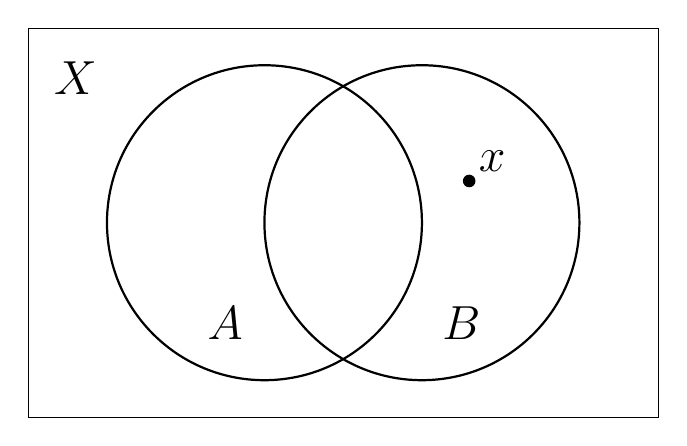
\begin{tikzpicture}[outline/.style={draw=#1,thick}]
\draw[fill=none] (0,0) rectangle (8,4.94);
%\fill[red!60,outline=red] (3,2.47) circle (2);
\fill[fill=none,outline=black] (3,2.47) circle (2);
%\begin{scope}
%\pgfsetfillopacity{0.5}
%\fill[blue,outline=blue] (5,2.47) circle (2);
\fill[fill=none,outline=black] (5,2.47) circle (2);
%\end{scope}
\draw (.6,4.3) node {\LARGE $X$};
\draw (2.5,1.2) node {\textcolor{black}{\LARGE $A$}};
\draw (5.5,1.2) node {\textcolor{black}{\LARGE $B$}};
\coordinate [label=60:\textcolor{black}{\LARGE $x$}] (x) at (5.6,3);
\fill[black] (x) circle (.08);
\end{tikzpicture}

\end{center}

Jos kaikki joukon $A$ alkiot ovat myös joukon $B$ alkioita, niin joukkoa $A$ kutsutaan joukon $B$ \termi{osajoukko}{osajoukoksi}. Osajoukkoa merkitään $A\subset B$. 

%{\bf KUVA}

\begin{center}

%%  Kuva s. 55

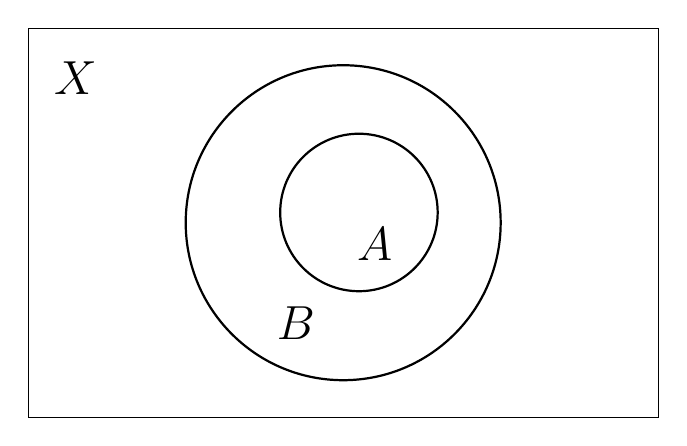
\begin{tikzpicture}[outline/.style={draw=#1,thick}]
\draw[fill=none] (0,0) rectangle (8,4.94);
%\fill[red!60,outline=red] (4,2.47) circle (2);
\fill[fill=none,outline=black] (4,2.47) circle (2);
%\begin{scope}
%\pgfsetfillopacity{0.5}
%\fill[blue,outline=blue] (4.2,2.6) circle (1);
\fill[fill=none,outline=black] (4.2,2.6) circle (1);
%\end{scope}
\draw (.6,4.3) node {\LARGE $X$};
\draw (4.4,2.2) node {\textcolor{black}{\LARGE $A$}};
\draw (3.4,1.2) node {\textcolor{black}{\LARGE $B$}};
\end{tikzpicture}

\end{center}

Jos $A\subset B$ ja $B\subset A$, niin  $A$ ja $B$ ovat sama joukko. Tällöin merkitään $A=B$. Samuus tarkoittaa sitä, että kyseisillä joukoilla on samat alkiot. % {\bf (toistoa, mitä pitäisikö siirtää aikaisemmaksi)}

%{\bf Esimerkki 1.}
\begin{esimerkki}
Akaan kaupunki muodostuu Toijalan, Viialan ja Kylmäkosken
kylistä. Akaa taas on osa Pirkanmaan maakuntaa. Olkoot $A
= \{\textrm{akaalaiset}\}$, $T = \{\textrm{toijalalaiset}\}$, $V
= \{\textrm{viialalaiset}\}$, $K = \{\textrm{kylmäkoskelaiset}\} $ ja $P = \{\textrm{pirkanmaalaiset}\}$. Onko lause tosi?

\begin{enumerate}[a)]
\item $V \subset A$
\item $A \subset T$
\item $A \subset P$
\item $K \subset P$
\end{enumerate}

%(Sopiva kuva/kartta?)

{\bf Ratkaisu.}
a) Kaikki viialalaiset ovat akaalaisia, joten lause on
tosi.

b) Lauseen mukaan kaikki akaalaiset ovat toijalalaisia.
Lause on epätosi.

c) Kaikki akaalaiset ovat pirkanmaalaisia, joten lause on
tosi.

d) Lauseen mukaan kaikki kylmäkoskelaiset ovat
pirkanmaalaisia. Koska kylmäkoskelaiset ovat akaalaisia
ja akaalaiset pirkanmaalaisia, niin lause on tosi.

{\bf Vastaus:} a) On. b) Ei ole. c) On. d) On.
\end{esimerkki}

\subsection*{Komplementti}
Ne perusjoukon $X$ alkiot, jotka eivät kuulu joukkoon $A$, muodostavat joukon $A$ \termi{komplementti}{komplementin}. Joukon $A$ komplementtia merkitään $\complement A$.

\begin{center}
%%  Ylempi kuva s. 56

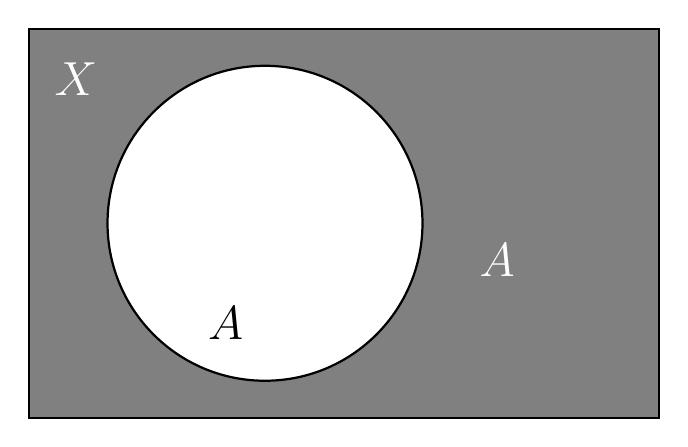
\begin{tikzpicture}[outline/.style={draw=#1,thick}]
\draw[fill=gray,outline=black] (0,0) rectangle (8,4.94);
\fill[white,outline=black] (3,2.47) circle (2);
\draw (.6,4.3) node {\textcolor{white}{\LARGE $X$}};
\draw (2.5,1.2) node {\textcolor{black}{\LARGE $A$}};
\coordinate [label=right:\textcolor{white}{\LARGE $\complement A$}] (x) at (5.6,2);
\end{tikzpicture}


\end{center}

Perusjoukon $X$ komplementti on \termi{tyhjä joukko}{tyhjä joukko}, jota merkitään $\emptyset$. Tyhjässä joukossa ei ole alkioita. Erityisesti tyhjä joukko on minkä tahansa joukon osajoukko.

%{\bf KUVA}

Joukkojen $A$ ja $B$ \termi{leikkaus}{leikkaus} $A\cap B$ on niiden perusjoukon alkioiden joukko, jotka kuuluvat sekä joukkoon $A$ että joukkoon $B$. Leikkausta voidaan havainnollistaa Venn-diagrammilla:

\begin{center}
%%  Alempi kuva s. 56

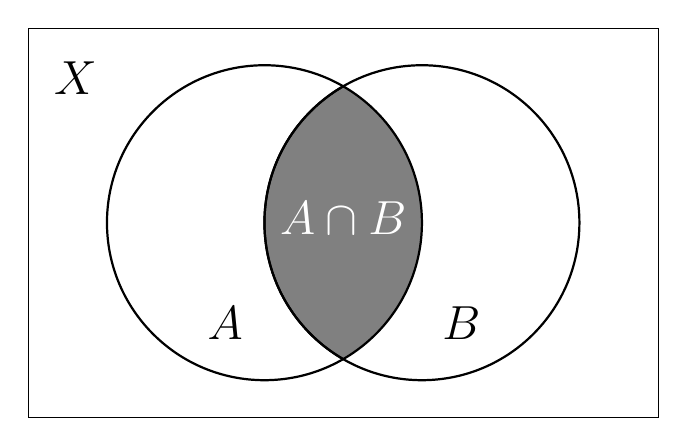
\begin{tikzpicture}[outline/.style={draw=#1,thick}]
\draw[fill=none] (0,0) rectangle (8,4.94);
\begin{scope}
\clip (3,2.47) circle (2);
\fill[gray,outline=black] (5,2.47) circle (2);
\end{scope}
\fill[fill=none,outline=black] (3,2.47) circle (2);
\fill[fill=none,outline=black] (5,2.47) circle (2);
\draw (.6,4.3) node {\LARGE $X$};
\draw (2.5,1.2) node {\textcolor{black}{\LARGE $A$}};
\draw (5.5,1.2) node {\textcolor{black}{\LARGE $B$}};
\coordinate [label=90:\textcolor{white}{\LARGE $A\cap B$}] (x) at (4,2.2);
\end{tikzpicture}

\end{center}

%{\bf KUVA}

Joukkojen $A$ ja $B$ \termi{yhdiste}{yhdiste} $A\cup B$ muodostuu niistä perusjoukon alkioista, jotka kuuluvat jompaankumpaan joukoista $A$ ja $B$. 
Joukkojen yhdistettä voidaan jälleen havainnollistaa Venn-diagrammin avulla:

\begin{center}
%%  Ylempi kuva s. 57

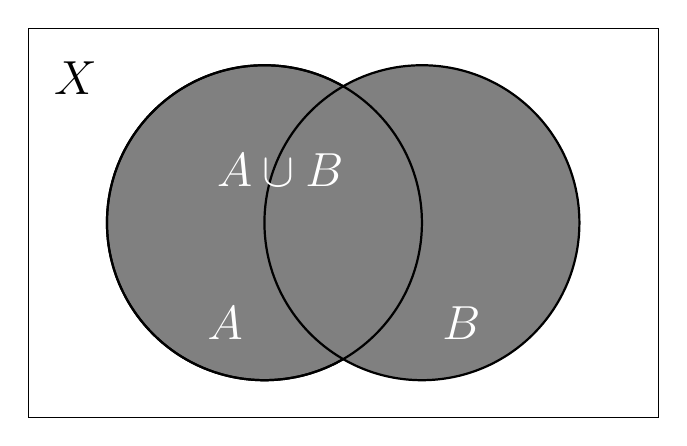
\begin{tikzpicture}[outline/.style={draw=#1,thick}]
\draw[fill=none] (0,0) rectangle (8,4.94);
\fill[fill=gray,outline=black] (3,2.47) circle (2);
\fill[fill=gray,outline=black] (5,2.47) circle (2);
\fill[fill=none,outline=black] (3,2.47) circle (2);
\draw (.6,4.3) node {\LARGE $X$};
\draw (2.5,1.2) node {\textcolor{white}{\LARGE $A$}};
\draw (5.5,1.2) node {\textcolor{white}{\LARGE $B$}};
\coordinate [label=90:\textcolor{white}{\LARGE $A\cup B$}] (x) at (3.2,2.8);
\end{tikzpicture}

\end{center}

%{\bf KUVA}

%(Venn-diagrammit, matemaattisen väitteen totuus, avoin lause)

Joukkojen $A$ ja $B$ \termi{erotus}{erotuksella} tarkoitetaan joukkoa, joka jää jäljelle, kun joukosta $A$ poistetaan kaikki joukon $B$ alkiot. Tätä joukkoa merkitään $A\setminus B$. 

\begin{center}
%%  Alempi kuva s. 57

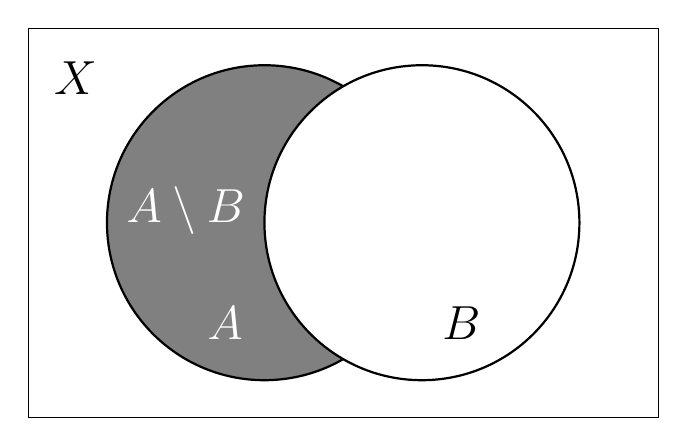
\begin{tikzpicture}[outline/.style={draw=#1,thick}]
\draw[fill=none] (0,0) rectangle (8,4.94);
\fill[fill=gray,outline=black] (3,2.47) circle (2);
\fill[fill=white,outline=black] (5,2.47) circle (2);
\draw (.6,4.3) node {\LARGE $X$};
\draw (2.5,1.2) node {\textcolor{white}{\LARGE $A$}};
\draw (5.5,1.2) node {\textcolor{black}{\LARGE $B$}};
\coordinate [label=90:\textcolor{white}{\LARGE $A\setminus B$}] (x) at (2,2.2);
\end{tikzpicture}

\end{center}


%{\bf Esimerkki 2.}
\begin{esimerkki}
Olkoot $A = \{0, 1, 2, 3, 4, 5, 6\}$ ja $B = \{2, 4, 6, 8, 10\}$. Määritä joukot a) $A\cup B$ b) $A \cap B$ c) $A\setminus B$ d) $B \setminus A$.

{\bf Ratkaisu:} 
a) Joukkojen $A$ ja $B$ yhdisteeseen $A \cup B$ kuuluvat ne alkiot, jotka kuuluvat jompaankumpaan joukoista $A$ ja $B$. Siten $A\cup B = \{0, 1, 2, 3, 4, 5, 6, 8, 10\}$.

b) Joukkojen $A$ ja $B$ leikkaukseen $A \cap B$ kuuluvat ne alkiot, jotka kuuluvat sekä joukkoon $A$ että joukkoon $B$. Siten $A \cap B = \{2, 4, 6\}$.

c) Joukkojen $A$ ja $B$ erotukseen $A \setminus B$ kuuluvat ne alkiot, jotka kuuluvat joukkoon $A$, mutta eivät joukkoon $B$. Siten $A \setminus B = \{0, 1, 3, 5\}$.

d) Vastaavasti erotukseen $B \setminus A$ kuuluvat ne alkiot, jotka kuuluvat joukkoon $B$, mutta eivät joukkoon $A$. Siten $B \setminus A = \{8, 10\}$.

{\bf Vastaus:} a) $A \cup B = \{0, 1, 2, 3, 4, 5, 6, 8, 10\}$,  b) $A \cap B = \{2, 4, 6\}$,  c) $A \setminus B = \{0, 1, 3, 5\}$,  d) $B \setminus A = \{8, 10\}$.
\end{esimerkki}


%{\bf Esimerkki 3.}
\begin{esimerkki}
Koulussa on $700$ opiskelijaa. Erään kyselyn tuloksena saatiin selville, että $550$ heistä 
seuraa uutisia säännöllisesti sanomalehdistä ja $400$ Internetistä. Opiskelijoista $350$  
seuraa uutisia säännöllisesti kummastakin lähteestä. Havainnollista tilannetta Venn-diagrammilla ja vastaa seuraaviin kysymyksiin.
\begin{enumerate}[a)]
\item Kuinka moni opiskelija seuraa uutisia vain Internetistä?
\item Kuinka moni opiskelija ei seuraa uutisia ollenkaan?
\end{enumerate}

{\bf Ratkaisu:}

%[Venn-diagrammi]		
\begin{center}


%%  Kuva s. 58....onko tämä kuten pitää?

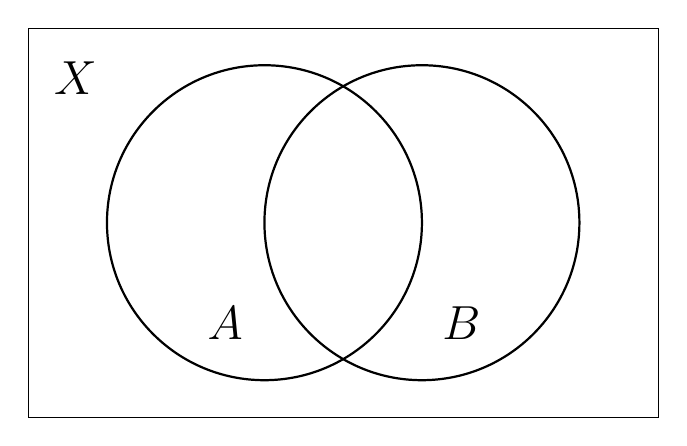
\begin{tikzpicture}[outline/.style={draw=#1,thick}]
\draw[fill=none] (0,0) rectangle (8,4.94);
\fill[fill=none,outline=black] (3,2.47) circle (2);
\begin{scope}
\pgfsetfillopacity{0.5}
\fill[fill=none,outline=black] (5,2.47) circle (2);
\end{scope}
\draw (.6,4.3) node {\LARGE $X$};
\draw (2.5,1.2) node {\textcolor{black}{\LARGE $A$}};
\draw (5.5,1.2) node {\textcolor{black}{\LARGE $B$}};
\end{tikzpicture}

\end{center}

Perusjoukko $X$ sisältää kaikki koulun opiskelijat. Joukkoon $A$ kuuluvat opiskelijat, jotka seuraavat uutisia sanomalehdistä, ja joukkoon $B$ opiskelijat, jotka seuraavat uutisia Internetistä.

a) Opiskelijoista $400$ seuraa uutisia Internetistä ja $350$ heistä seuraa uutisia myös sanomalehdistä. Näin ollen $400 - 350 = 50$ opiskelijaa seuraa uutisia vain Internetistä. Tämä on joukon $B \setminus A$ alkioiden lukumäärää. 

b) Ainakin toisesta lähteestä uutisia seuraa $550 + 400 - 350 = 600$ opiskelijaa. Tällöin $700 - 600 = 100$ opiskelijaa ei seuraa uutisia ollenkaan. Tämä on joukon $\compl(A\cup B)$ alkioiden lukumäärä.

{\bf Vastaus:} a) $50$ opiskelijaa b) $100$ opiskelijaa
\end{esimerkki}


\begin{esimerkki}
%{\bf Esimerkki 4.}
Olkoot perusjoukko $\R$ sekä joukot $A$ ja $B$ reaalilukuvälit $A = ]-5, 1]$ ja $B = ]-2, 4]$. Ilmaise välimerkintää käyttäen joukot a) $A\cup B$, b) $A \setminus B$, c) $\compl A$, d) $\compl( A \cap B)$. %{\bf (lukusuora jonnekin?)}  

{\bf Ratkaisu:} 
\begin{enumerate}[a)]
\item Joukkojen $A$ ja $B$ yhdisteeseen $A \cup B$ kuuluvat ne luvut, jotka kuuluvat jompaankumpaan joukoista $A$ ja $B$. Siten $A\cup B = ]-5, 4]$.
\item Joukkojen $A$ ja $B$ erotukseen $A \setminus B$ kuuluvat ne luvut, jotka kuuluvat joukkoon $A$, mutta eivät joukkoon $B$. Siten $A \setminus B = ]-5, -2]$.
\item Joukon $A$ komplementtiin $\compl A$ kuuluvat ne reaaliluvut, jotka eivät kuulu joukkoon $A$. Komplementti muodostuu väleistä $]-\infty, -5]$ ja $]1, \infty [$. Siten $\compl A = ]-\infty, -5] \cup ]1, \infty [$.
\item Joukkojen $A$ ja $B$ leikkaukseen kuuluvat ne luvut, joka kuuluvat sekä joukkoon $A$ että joukkoon $B$. Siten $A\cap B = ]-2, 1]$. Leikkauksen komplementtiin kuuluvat kaikki muut reaaliluvut, joten $\compl( A \cap B) = ]-\infty, -2] \cup ]1,\infty [$.
\end{enumerate}

{\bf Vastaus:}
\begin{enumerate}[a)]
\item $A\cup B =]-5, 4]$,
\item $A \setminus B = ]-5, -2]$,
\item $\compl A = ]-\infty, -5] \cup ]1, \infty [$,
\item $\compl( A \cap B) = ]-\infty, -2] \cup ]1,\infty [$.
\end{enumerate}
\end{esimerkki}

\begin{esimerkki}
%{\bf Esimerkki 5.}
Osoita Venn-diagrammia käyttäen, että $\compl A \cap B = B \setminus A$.

{\bf Ratkaisu:}

%[Venn-diagrammi, jossa on esitetty $\compl A \cap B$]

\begin{center}
%%  Kuva s. 59

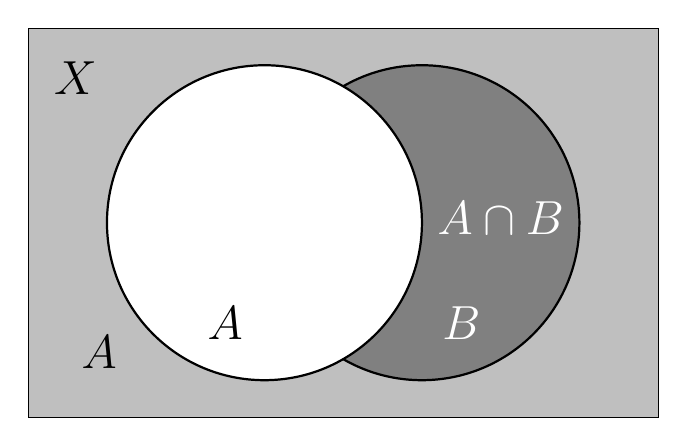
\begin{tikzpicture}[outline/.style={draw=#1,thick}]
\draw[fill=gray!50] (0,0) rectangle (8,4.94);
\fill[fill=gray,outline=black] (5,2.47) circle (2);
\fill[fill=white,outline=black] (3,2.47) circle (2);
\draw (.6,4.3) node {\LARGE $X$};
\draw (2.5,1.2) node {\textcolor{black}{\LARGE $A$}};
\draw (5.5,1.2) node {\textcolor{white}{\LARGE $B$}};
\coordinate [label=90:\textcolor{white}{\LARGE $\complement A\cap B$}] (x) at (6,2.2);
\coordinate [label=90:\textcolor{black}{\LARGE $\complement A$}] (y) at (.9,.5);
\end{tikzpicture}


\end{center}

Joukon $A$ komplementtijoukko $\compl A$ on niiden perusjoukon alkioiden joukko, jotka eivät kuulu joukkoon $A$, ja $\compl A\cap B$ on tämän joukon leikkaus joukon $B$ kanssa.

%[Venn-diagrammi, jossa on esitetty $B \setminus A$]

\begin{center}

%%  Kuva s. 60

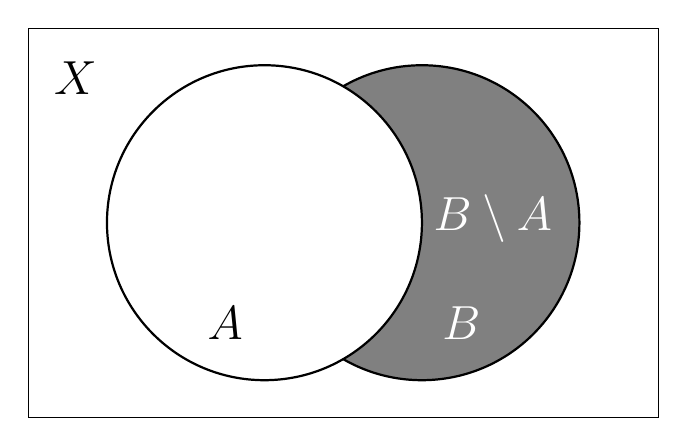
\begin{tikzpicture}[outline/.style={draw=#1,thick}]
\draw[fill=none] (0,0) rectangle (8,4.94);
\fill[fill=gray,outline=black] (5,2.47) circle (2);
\fill[fill=white,outline=black] (3,2.47) circle (2);
\draw (.6,4.3) node {\LARGE $X$};
\draw (2.5,1.2) node {\textcolor{black}{\LARGE $A$}};
\draw (5.5,1.2) node {\textcolor{white}{\LARGE $B$}};
\coordinate [label=90:\textcolor{white}{\LARGE $B\setminus A$}] (x) at (5.9,2.1);
\end{tikzpicture}


\end{center}

Joukko $B \setminus A$ sisältää ne joukon $B$ alkiot, jotka eivät kuulu joukkoon $A$.
Venn-diagrammit havainnollistavat, että on kyse samasta joukosta. Siis $\compl A\cap B = B \setminus A$.
\end{esimerkki}

%\newpage


%\section*{Tehtäviä}

\Harjoitustehtavat

\begin{enumerate}

\item Onko lause tosi?
\begin{enumerate}[a)]
\item $K \subset A$
\item $A \subset V$
\item $V \subset P$
\item $V \subset T$
\end{enumerate}
Merkinnät ovat samat kuin esimerkissä 1.

\item Olkoot $A = \{7, 8, 9\}$ ja $B=\{5, 6, 7\}$. Määritä joukot
\begin{enumerate}[a)]
\item $A \cup B$,
\item $A \cap B$,
\item $A \setminus B$,
\item $B \setminus A$.
\end{enumerate}

\item Olkoot perusjoukko $X$ aakkoset, $A$ vokaalit ja $B=\{x, y, z\}$.
Määritä joukot
\begin{enumerate}[a)]
\item $B\setminus A$,
\item $A\cap B$,
\item $\complement A$,
\item $A \setminus X$.
\end{enumerate}


\item
Olkoot $A$ koulussa opiskelevien täysi-ikäisten opiskelijoiden joukko ja $B$ niiden opiskelijoiden joukko, jotka asuvat vanhempiensa luona. Millaiset opiskelijat kuuluvat joukkoon a) $A \cap B$,  b) $\compl A$, c) $A \cup \compl B$, d) $A\setminus B$, e) $B \setminus A$, f) $\compl (A \cup B)$?

\item
Ilmaise joukkomerkintöjä käyttäen kuvan
\begin{enumerate}[a)]
\item keltainen alue,
\item sininen alue,
\item violetti alue,
\item vihreä alue.
\end{enumerate}

\begin{center}

%%  Kuva s. 62

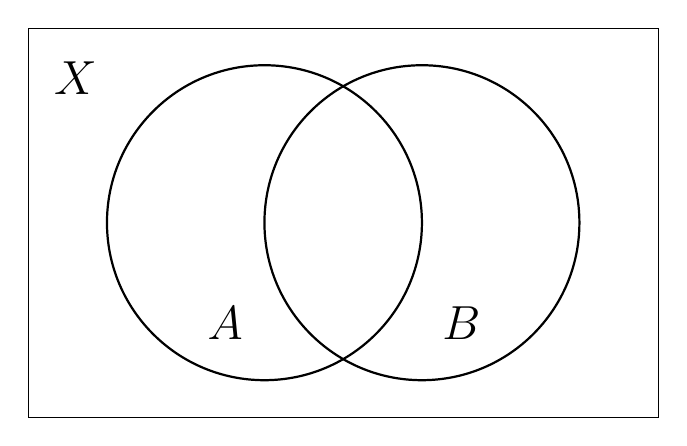
\begin{tikzpicture}[outline/.style={draw=#1,thick}]
\draw[fill=none] (0,0) rectangle (8,4.94);
\fill[fill=none,outline=black] (3,2.47) circle (2);
\begin{scope}
\pgfsetfillopacity{0.5}
\fill[fill=none,outline=black] (5,2.47) circle (2);
\end{scope}
\draw (.6,4.3) node {\LARGE $X$};
\draw (2.5,1.2) node {\textcolor{black}{\LARGE $A$}};
\draw (5.5,1.2) node {\textcolor{black}{\LARGE $B$}};
\end{tikzpicture}

\end{center}
%PICXX2

\item
Olkoot $A \cap B$, $A \setminus B$ ja $B \setminus A$ epätyhjiä joukkoja. Esitä Venn-diagrammissa varjostettuna alue, joka kuvaa joukkoa a) $\compl (A \cup B)$, b) $\compl (A \cap B)$, c) $\compl B \cap A$.

\item Luokalla on 30 opiskelijaa. Heistä 14 harrastaa jääkiekkoa, 12 jalkapalloa ja 3 molempia. 
\begin{enumerate}[a)]
\item Kuinka moni opiskelija harrastaa pelkkää jääkiekkoa?
\item Kuinka moni opiskelija harrastaa pelkkää jalkapalloa?
\item Kuinka moni opiskelija ei harrasta kumpaakaan?
\end{enumerate}
Vihje: Tilanteesta kannattaa piirtää Venn-diagrammi.

\item Olkoot perusjoukko $\R$ sekä joukot $A$ ja $B$ reaalilukuvälit $A=[1, 5]$ ja $B=[3, 6]$. Ilmaise välimerkintää käyttäen joukot
\begin{enumerate}[a)]
\item $A \cap B$,
\item $A \cup B$,
\item $A \setminus B$,
\item $\compl A$.
\end{enumerate}

\item Yhdistä samaa tarkoittavat lauseet.
\[
\begin{array}{llll}
A & (x\in A)\land (x\in B) & 1 & x\in \complement A \\
B & x\notin A & 2 & x \in A\setminus B \\
C & (x\in A)\lor (x\in B) & 3 & x\in (A\cap B) \\
D & (x\in A)\land (x\notin B) & 4 & x\in (A\cup B)
\end{array}
\]

\item Osoita Venn-diagrammin avulla, että
\begin{enumerate}[a)]
\item 
\[
A\cup (B \cap C) = (A\cup B)\cap(A\cup C),
\]
\item 
\[
A\cap (B \cup C) = (A\cap B)\cup(A\cap C).
\]
\end{enumerate}

\item Sievennä Venn-diagrammin avulla.
\begin{enumerate}[a)]
\item $(B\cap A) \cup (B \cap \compl A)$
\item $\compl (A\cup B) \cup (A \setminus B) \cup (B \setminus A)$
\end{enumerate}

\item
Olkoot perusjoukko kokonaislukujen joukko $\Z$, $W$ parillisten kokonaislukujen joukko ja $Y$ luvulla $3$ jaollisten kokonaislukujen joukko. Näitä joukkoja voidaan merkitä $W = \{2n\,|\, n\in\Z\}$ ja $Y = \{3n \,|\, n \in \Z\}$. Määritä joukot a) $W \cap Y$, b) $W \setminus Y$, c) $W \cup Y$.

\item Onko lause tosi?
\begin{enumerate}[a)]
\item $\sqrt{2} \in \R$
\item $-3 \in \N$
%\item $\Z \subset \Q$
\item $\pi \in \R \setminus \Q$
\item $\frac{4}{2} \in \Q \setminus \Z$
\item $\emptyset \subset \Z$
\end{enumerate}

\item Määritä joukon a) $\{1, 2\}$ b) $\{1, 2, 3\}$ kaikki osajoukot.

\item * %(Lisämateriaalia)
Joukon $A$ \termi{potenssijoukko}{potenssijoukoksi} $\mathcal{P}(A)$ kutsutaan kaikkien joukon $A$ osajoukkojen muodostamaa joukkoa:
\[
\mathcal{P}(A)=\{ B \, | \, B\subset A\}.
\]
\begin{enumerate}[a)]
\item Määritä joukon $\{1, 2, 3\}$ potenssijoukko.
\item Määritä tyhjän joukon $\emptyset$ potenssijoukko.
\item Joukko $\{\emptyset\}$ on joukko, jonka ainut alkio on tyhjä joukko. Määritä joukon $\{\emptyset\}$ potenssijoukko.
\end{enumerate}

\item * %(Lisämateriaalia)
Luonnolliset luvut voidaan tulkita joukko-opillisesti käyttämällä edellisessä tehtävässä esitettyä potenssijoukon käsitettä. Ajatuksena on, että lukua $0$ vastaa tyhjä joukko $\emptyset$ ja kutakin luonnollista lukua $n + 1$ vastaava joukko on luonnollista lukua $n$ vastaavan joukon potenssijoukko. Siis esimerkiksi lukua $1$ vastaa tyhjän joukon $\emptyset$ potenssijoukko $\mathcal{P}(\emptyset)$, lukua $2$ potenssijoukko $\mathcal{P}(\mathcal{P}(\emptyset))$ ja niin edelleen.
\begin{enumerate}[a)]
\item Määritä lukuja $3$ ja $4$ vastaavat joukot.
\item Mitä luonnollista lukua vastaa joukko $\{\emptyset,\{\emptyset\}\}$?
\item Vastaako joukko $\{\{\emptyset\}\}$ jotakin luonnollista lukua? Miksi?
\end{enumerate}

\end{enumerate}

\subsection*{Kotitehtäviä}

\begin{enumerate}

\item Olkoot $A = \{a, b, c, d\}$ ja $B=\{a, c, e\}$. Määritä joukot
\begin{enumerate}[a)]
\item $A \cup B$, 
\item $A \cap B$,
\item $A \setminus B$,
\item $B \setminus A$.
\end{enumerate}

\item Onko lukujoukkoja koskeva lause tosi?
\begin{enumerate}[a)]
\item $\Z \subset \N$
\item $\Z \subset \Q$
\item $\R \subset \Z$
\item $\Q \subset \N$
\item $\Q \subset \Q$
\end{enumerate}

\item Olkoot perusjoukko $X$ aakkoset, $A=\{j, o, k, u\}$, $B=\{k, o, j, u\}$ ja $C=\{k, a, j, o\}$. Määritä joukot
\begin{enumerate}[a)]
\item $A\setminus B$,
\item $(A\cap B)\cup C$,
\item $A\setminus \complement (B\cup C)$.
\end{enumerate}

\item Olkoot $X$ perusjoukko ja $A$ jokin perusjoukon osajoukko. Sievennä.
\begin{enumerate}[a)]
\item $A\cup \emptyset$
\item $A\cap \emptyset$
\item $A\cap X$
\item $A\cup X$
\end{enumerate}

\item
Olkoot $A \subset B$ ja $B \setminus A$ epätyhjä. Esitä Venn-diagrammissa varjostettuna alue, joka kuvaa joukkoa a) $B \setminus A$, b) $\compl A \cap B$, c) $A \cup \compl B$.

\item
Olkoon perusjoukko $X$ kaikkien kalenterivuoden päivien joukko. Olkoot $A$ arkipäivien (maanantai--perjantai) joukko, $L$ liputuspäivien joukko ja $T$ toukokuulle ajoittuvien päivien joukko. Millaiset päivät kuuluvat joukkoon
\begin{enumerate}[a)]
\item $\compl A$
\item $L \cap \compl T$
\item $L \setminus A$
\item $T \setminus (A \cup L)$
\item $\compl (A \cup L \cup T)$?
\end{enumerate}

\item Onko lause tosi?
\begin{enumerate}[a)]
\item $0 \in \{0, 1, 2\}$
\item $\{0\} \subset \{0, 1, 2\}$
\item $\emptyset \subset \{1, 2\}$
\item $\{\textrm{å}, \textrm{ä}, \textrm{ö}\} \subset \{\textrm{o}, \textrm{ä}, \textrm{ö}\}$
\end{enumerate}

\item Luokan opiskelijoista kahdeksalla on läppäri, kymmenellä pöytäkone ja
viidellä tabletti.
Kahdella opiskelijalla on sekä läppäri että pöytäkone, kolmella sekä
tabletti että pöytäkone, mutta kellään ei ole sekä läppäriä että
tablettia. Kahdella opiskelijalla ei ole mitään tietokonetta.
\begin{enumerate}[a)]
\item Piirrä tilannetta kuvaava Venn-diagrammi.
\item Kuinka monella opiskelijalla on läppäri mutta ei pöytäkonetta?
\item Kuinka monella opiskelijalla on vain pöytäkone?
\item Kuinka monta opiskelijaa luokalla on?
\end{enumerate}

\item Olkoot perusjoukko $\R$ sekä joukot $A$ ja $B$ reaalilukuvälit $A=]-1, 2[$ ja $B=[0, 4[$. Ilmaise välimerkintää käyttäen joukot
\begin{enumerate}[a)]
\item $A \cup B$,
\item $A \cap B$,
\item $\compl (A \cap B)$,
\item $B \setminus A$,
\item $B \setminus (A \cap B)$,
\item $A \cap \compl B$.
\end{enumerate}

\item Osoita Venn-diagrammin avulla, että
\begin{enumerate}[a)]
\item 
\[
X\setminus (A\cup B) = (X\setminus A)\cap (X\setminus B),
\]
\item 
\[
X \setminus (A\cap B) = (X\setminus A)\cup (X\setminus B).
\]
\end{enumerate}

\item Jos $A\subset B$ ja $B\subset C$, niin mitä voidaan päätellä joukoista $A$ ja $C$? Perustele 
\begin{enumerate}[a)]
\item Venn-diagrammin avulla,
\item osajoukon määritelmän avulla.
\end{enumerate}

\item
Onko lause tosi?
\begin{enumerate}[a)]
\item $A \cap B \subset A$
\item $\compl (\compl A) = A$
\item $(A\cup B) \setminus B = A$
\item $A \cap \compl B = A \setminus B$
\item $B \cap \compl B = B$
\end{enumerate}

\item Merkitään kuvan ympyröiden sisään jääviä joukkoja kirjaimilla $A$, $B$ ja $C$. Ilmaise joukkomerkintöjä käyttäen joukkojen $A$, $B$ ja $C$ avulla kuvan
\begin{enumerate}[a)]
\item alue $D$,
\item alue $E$,
\item alue $F$,
\item alue $G$.
\end{enumerate}

\medskip

\begin{center}
% Kuva s. 66, MUUTA TEHTÄVÄ VASTAAMAAN KUVAA

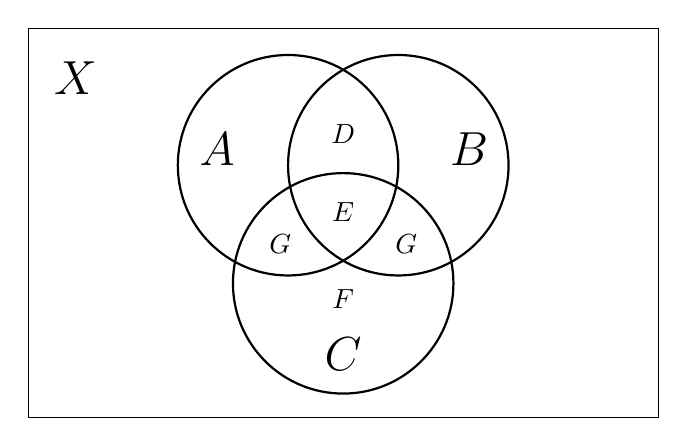
\begin{tikzpicture}[outline/.style={draw=#1,thick}]
\draw[fill=none] (0,0) rectangle (8,4.94);
\fill[fill=none,outline=black] (3.3,3.2) circle (1.4);
\fill[fill=none,outline=black] (4.7,3.2) circle (1.4);
\fill[fill=none,outline=black] (4,1.7) circle (1.4);
\draw (.6,4.3) node {\LARGE $X$};
\draw (2.4,3.4) node {\LARGE $A$};
\draw (5.6,3.4) node {\LARGE $B$};
\draw (4,.8) node {\LARGE $C$};
\draw (4,3.6) node {$D$};
\draw (4,2.6) node {$E$};
\draw (4,1.5) node {$F$};
\draw (3.2,2.2) node {$G$};
\draw (4.8,2.2) node {$G$};
\end{tikzpicture}


\end{center}
%PICXX3

\medskip

\item Tarkastellaan kaksinumeroisia luonnollisia lukuja $10, 11, \ldots, 98, 99$.
\begin{enumerate}[a)]
\item Kuinka monta kaksinumeroista luonnollista lukua on olemassa?
\item Kuinka moni niistä on jaollinen luvulla $4$? Kuinka moni ei ole jaollinen luvulla $4$?
\item Kuinka moni kaksinumeroisista luonnollisista luvuista on jaollinen luvulla $6$?
\item Kuinka moni kaksinumeroisista luonnollisista luvuista on jaollinen luvuilla $4$ ja $6$?
\item Kuinka moni kaksinumeroisista luonnollisista luvuista on jaollinen luvulla $4$ tai luvulla $6$?
\item Kuinka moni kaksinumeroisista luonnollisista luvuista ei ole jaollinen luvulla $4$ eikä luvulla $6$?
\item Piirrä tilanteesta Venn-diagrammi.
\end{enumerate}

\end{enumerate}

\newpage


\section{Avoin lause ja konnektiivien joukko-opillinen tulkinta.}

\subsection*{Tutkimustehtävä}
\begin{enumerate}
\item Ketkä seuraavista henkilöistä toteuttavat väitteen ''henkilö on entinen Suomen tasavallan presidentti''? 
a) Urho Kekkonen,  b)  Paavo Nurmi,  c)  Armi Kuusela,  d)  Tarja Halonen,  
e) Carl Gustaf Emil Mannerheim.
\item
Lause $P(x)$ on ''$-10x = 100$''. Onko lause $P(-2)$, $P(5)$ tai $P(-10)$ tosi?
\item
Millä kokonaisluvuilla lause $Q(x)$: ''$2x^2 - x - 1 = 0$'' on tosi?
\end{enumerate}

\subsection*{Avoin lause ja ratkaisujoukko}
Lauselogiikassa asioiden tiloja ilmaisemaan käytetään atomilauseita, esimerkiksi lausetta $S$: ''sataa''. Tämän lauseen totuusarvo kuitenkin riippuu tarkastelijan olinpaikasta $x$. Onkin luonnollinen ajatus tarkastella loogista lausetta, jossa on \termi{vapaa muuttuja}{vapaa muuttuja}, tässä tapauksessa paikka $x$. Tällöin merkitään $S(x)$: ''paikassa $x$ sataa''. Lauseen totuusarvo ratkeaa vasta, kun vapaan muuttujan arvo kiinnitetään. Siksi lausetta $S(x)$ kutsutaan \termi{avoin lause}{avoimeksi lauseeksi}. Avoimia lauseita kutsutaan myös \termi{predikaatti}{predikaateiksi}, ja avoimia lauseita käsittelevää logiikkaa sanotaan \termi{predikaattilogiikka}{predikaattilogiikaksi}.

Vapaa muuttuja saa arvoja annetusta perusjoukosta $X$. Perusjoukkoa ei ole tapana kirjoittaa näkyviin, jos se voidaan päätellä tilanteesta. Esimerkiksi yllä mainitussa avoimessa lauseessa $S(x)$ perusjoukkona ovat kaikki paikkakunnat. Avoimen lauseen \termi{ratkaisujoukko}{ratkaisujoukon} muodostavat puolestaan ne perusjoukon alkiot, joilla avoin lause on tosi. Esimerkiksi lauseen $S(x)$ ratkaisujoukkona ovat kaikki ne paikkakunnat, joilla sataa.

Avoimessa lauseessa voi olla useampiakin muuttujia, voitaisiin esimerkiksi tarkastella lausetta $S(x, t)$: ''paikassa $x$ sataa hetkellä $t$''. Monimutkaisempia avoimia lauseita voidaan muodostaa konnektiivien
avulla.

Matematiikassa avoin lause on usein yhtälö tai epäyhtälö. Yhtälössä esiintyvät tuntemattomat voidaan tulkita vapaiksi muuttujiksi. Esimerkiksi voidaan merkitä $C(x)$: ''$\cos x + x^2= 2$''. Avoimen lauseen ratkaisujoukko on niiden pisteiden $x$ joukko, joilla kyseinen yhtälö toteutuu.

\begin{esimerkki}
%{\bf Esimerkki 1.}
Olkoon $P(x)$ avoin lause ''$2x - 10 = 0$''. Onko lause a) $P(5)$, b) $P(-5)$ tosi?

{\bf Ratkaisut:}

a) Sijoitetaan luku $5$ avoimeen lauseeseen muuttujan $x$ paikalle. Koska $2\cdot 5 - 10 = 10 - 10 = 0$, lause $P(5)$ on tosi.

b) Sijoitetaan luku $-5$ avoimeen lauseeseen muuttujan $x$ paikalle. Koska $2\cdot(-5) - 10 = -10 - 10 = -20 \neq 0$, lause $P(-5)$ on epätosi.

{\bf Vastaukset:} a) On. b) Ei ole.
\end{esimerkki}

\begin{esimerkki}
%{\bf Esimerkki 2.}
Yhtälöiden ja epäyhtälöiden yhteydessä perusjoukkoa kutsutaan myös \termi{määrittelyjoukko}{määrittelyjoukoksi}. Ratkaise avoin lause $2x^2 + 5x - 3 < 0$, kun määrittelyjoukko on a) reaalilukujen joukko b) kokonaislukujen joukko.

{\bf Ratkaisut:}

a) Tutkitaan polynomifunktion $2x^2 + 5x - 3$ merkkiä. Ratkaistaan funktion $2x^2 + 5x - 3$ nollakohdat toisen asteen yhtälön ratkaisukaavalla.
\[
2x^2 + 5x - 3 = 0
\]
\[
x =\frac{-5\pm\sqrt{5^2-4\cdot 2\cdot(-3)}}{2\cdot 2}
\] 
\[
x = \frac{-5\pm\sqrt{49}}{4} =\frac{-5\pm 7}{4}
\]
\[
x = -3\textrm{  tai  }x =\frac{1}{2}.
\]
Koska funktion $2x^2 + 5x - 3$ kuvaaja on ylöspäin aukeava paraabeli, avoin lause $2x^2 + 5x - 3 < 0$ toteutuu, kun $-3 < x < \frac{1}{2}$. Avoimen lauseen ratkaisujoukko on siis väli $]-3, \frac{1}{2}[$.

b) Kun määrittelyjoukko on kokonaislukujen joukko, a-kohdan ratkaisuista kelpaavat vain $x = -2$, $x = -1$ ja $x = 0$. Avoimen lauseen ratkaisujoukko on siis $\{-2, -1, 0\}$.

{\bf Vastaukset:} a) $-3 < x < \frac{1}{2}$, b) $x = -2$ tai $x = -1$ tai $x = 0$
\end{esimerkki}

\subsection*{Ominaisuudet ja osajoukot}
Jouk\-ko-opin soveltamisen kannalta on usein hyödyllistä \termi{samastus}{samastaa} keskenään joukot ja perusjoukon $X$ alkioiden ominaisuudet. Tällöin avoimelle lauseelle $P(x)$ käytetään myös merkintää $x\in P$. Jos $\lnot P(y)$, voidaan merkitä $y\notin P$. Tätä voidaan havainnollistaa Venn-diagrammilla. Kuvassa $x\in P$ ja $y\notin P$.

%{\bf kuva}.
\begin{center}
% Kuva s. 70

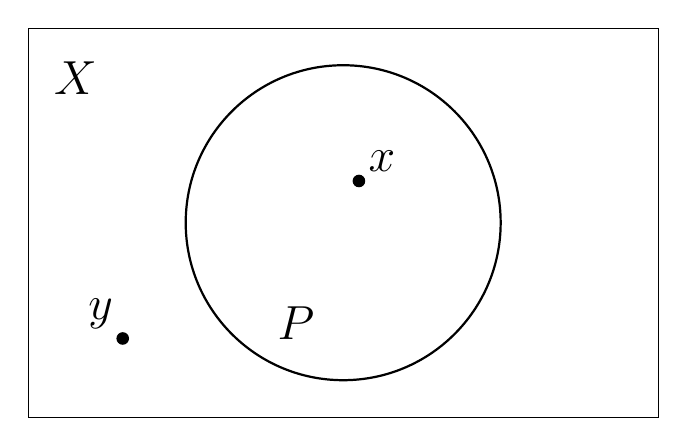
\begin{tikzpicture}[outline/.style={draw=#1,thick}]
\draw[fill=none] (0,0) rectangle (8,4.94);
\fill[fill=none,outline=black] (4,2.47) circle (2);
\draw (.6,4.3) node {\LARGE $X$};
\draw (3.4,1.2) node {\textcolor{black}{\LARGE $P$}};
\coordinate [label=60:\textcolor{black}{\LARGE $x$}] (x) at (4.2,3);
\fill[black] (x) circle (.08);
\coordinate [label=100:\textcolor{black}{\LARGE $y$}] (y) at (1.2,1);
\fill[black] (y) circle (.08);
\end{tikzpicture}


\end{center}

Jos predikaatit ajatellaan perusjoukon osajoukoiksi, niin joukko-opil\-li\-set operaatiot voidaan tulkita loogisina operaatioina. Kahden predikaatin $P$ ja $Q$ konjunktiota $P\land Q$ vastaa joukko-opissa leikkaus $P\cap Q$, disjunktiota $P \lor Q$ yhdiste $P\cup Q$ ja negaatiota $\lnot P$ komplementtijoukko $\complement P$. 
Tarkastellaan implikaation $P(x)\to Q(x)$ totuustaulua:

\bigskip

\begin{center}
\begin{tabular}{|c|c|c|}\hline
$x\in P$ & $x \in Q$ & $P(x) \to Q(x)$ \\ \hline
$1$ & $1$ & $1$\\ %\hline
$1$ & $0$ & $0$\\
$0$ & $1$ & $1$\\
$0$ & $0$ & $1$\\ \hline
\end{tabular}
\end{center}

\bigskip

Nähdään, että implikaatio on epätosi vain silloin, jos $x \in P$ mutta $x\not \in Q$, toisin sanoen $P$ ei ole $Q$:n osajoukko. Implikaatiota $P \to Q$ vastaa siis sisältymisrelaatio $P \subset Q$. Erityisesti periaatetta, että epätodesta lauseesta voidaan päätellä mitä tahansa, vastaa se, että tyhjä joukko $\emptyset$ on minkä tahansa joukon osajoukko. Ekvivalenssia $P\lequiv Q$ vastaava relaatio on joukko-opillinen yhtäsuuruus $P=Q$.

\begin{esimerkki}
%{\bf Esimerkki 3.}
 Olkoon perusjoukko kuviossa olevien nelikulmioiden joukko. Olkoot avoin lause $K(x)$: ''nelikulmio $x$ on suorakulmio'' ja $S(x)$: ''nelikulmio $x$ on suunnikas''. Ratkaise avoin lause.  a)  $K(x)$,  b)  $S(x)$,  c) $\lnot S(x)$,  d)  $\lnot K(x) \land S(x)$  e)  $K(x) \lequiv S(x)$.

\begin{center}
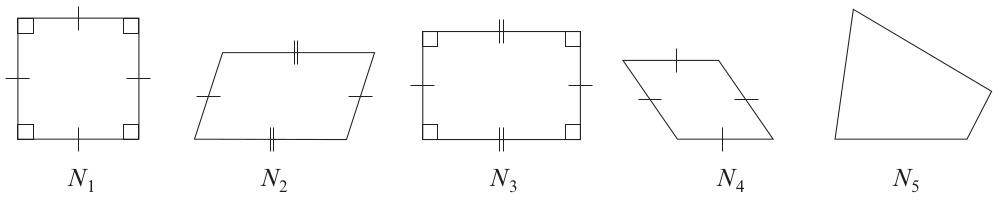
\includegraphics[width=10.1cm]{pictures/kpl3_2_esim3}
\end{center}


{\bf Ratkaisut:}

a) Avoin lause $K(x)$ on tosi, kun nelikulmio on suorakulmio. Suorakulmioita ovat nelikulmiot $N_1$ ja $N_3$, joten ratkaisujoukko on $\{ N_1, N_3\}$.

b) Avoin lause $S(x)$ on tosi, kun nelikulmio on suunnikas. Suunnikkaita ovat nelikulmiot $N_1$, $N_2$, $N_3$ ja $N_4$, joten ratkaisujoukko on $\{ N_1, N_2, N_3, N_4\}$.

c) Negaatio $\lnot S(x)$ on tosi, kun avoin lause $S(x)$ on epätosi eli kun nelikulmio ei ole suunnikas. Ehto toteutuu vain nelikulmiolla $N_5$. Ratkaisujoukko on $\{N_5\}$.

d) Avoin lause $\lnot K(x) \land S(x)$ on tosi, kun nelikulmio on suunnikas mutta ei suorakulmio. Ehto toteutuu nelikulmioilla $N_2$ ja $N_4$, joten ratkaisujoukko on $\{ N_2, N_4\}$.

e) Avoin lause $K(x) \lequiv S(x)$ on tosi, kun nelikulmio on suorakulmio ja suunnikas tai ei kumpikaan. Ehto toteutuu nelikulmioilla $N_1$, $N_3$ ja $N_5$, joten ratkaisujoukko on $\{ N_1, N_3, N_5\}$.

{\bf Vastaukset:}   a)  $\{ N_1, N_3\}$,   b)  $\{ N_1, N_2, N_3, N_4\}$,   c)  $\{N_5\}$,  d)  $\{ N_2, N_4\}$,  e)  $\{ N_1, N_3, N_5\}$.
\end{esimerkki}

\begin{esimerkki}
%{\bf Esimerkki 4.}
Heitetään kahta noppaa, punaista ja sinistä. Tuloksena saadaan lukupari $(x, y)$, missä $x$ on punaisen nopan silmäluku ja $y$ on sinisen nopan silmäluku. Perusjoukko $X$ sisältää lukuparit
\[
(1, 1), (1, 2), (1, 3), (1, 4), (1, 5), (1, 6), (2, 1), (2, 2),\ldots , (6, 5), (6, 6).
\]
Olkoot avoimet lauseet $S(x, y)$: ''$x + y > 9$'' ja $Y(x, y)$: ''$x = y$''. Määritä avoimen lauseen a) $S(x, y)$, b) $Y(x, y)$, c) $\lnot S(x, y) \land Y(x, y)$, d) $\lnot S(x, y) \to Y(x, y)$ ratkaisujoukko.

\begin{center}
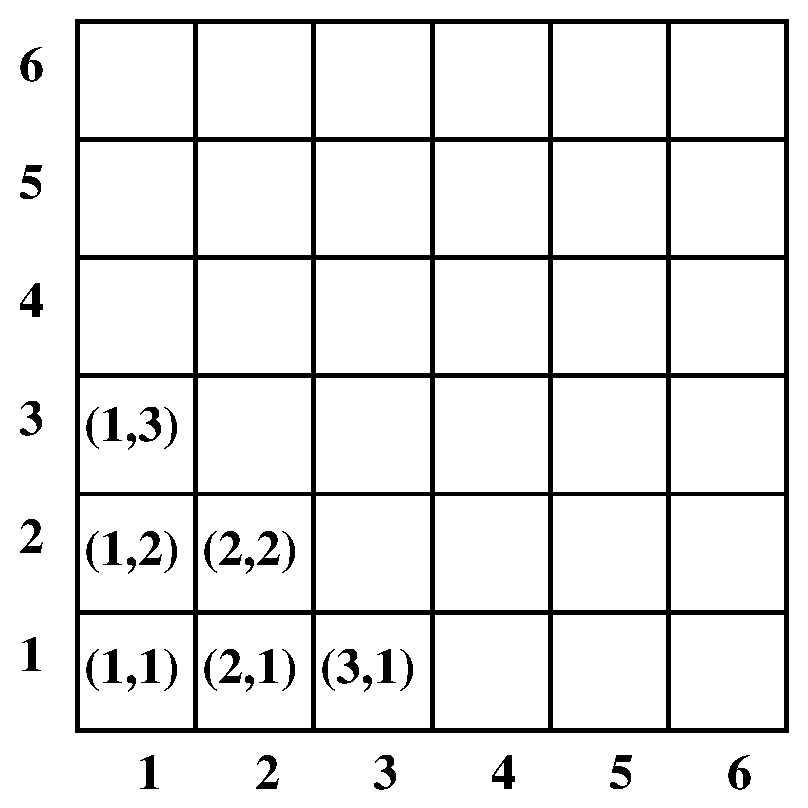
\includegraphics[width=5.3cm]{pictures/6x6}
\end{center}

{\bf Ratkaisu:}

a) Avoin lause $S(x, y)$ on tosi, kun noppien silmälukujen summa on suurempi kuin $9$ eli siis $10, 11$ tai $12$. Ehto toteutuu lukupareilla $(4, 6), (5, 5), (5, 6), (6, 4), (6, 5)$ ja $(6, 6)$. Ratkaisujoukko on
\[
\{(4, 6), (5, 5), (5, 6), (6, 4), (6, 5), (6, 6)\}.
\]

b) Avoin lause $Y(x, y)$ on tosi, kun noppien silmäluvut ovat samat. Ehto toteutuu lukupareilla $(1, 1), (2, 2), (3, 3), (4, 4), (5, 5)$ ja $(6, 6)$. Ratkaisujoukko on $\{(1, 1), (2, 2), (3, 3), (4, 4), (5, 5), (6, 6)\}$.

c) Avoin lause $\lnot S(x, y) \land Y(x, y)$ on tosi, kun noppien silmälukujen summa on pienempi tai yhtä suuri kuin $9$ ja kun silmäluvut ovat samat. Ehto toteutuu lukupareilla $(1, 1), (2, 2), (3, 3)$ ja $(4, 4)$. Ratkaisujoukko on $\{(1, 1), (2, 2), (3, 3), (4, 4)\}$.


d) Implikaatio $\lnot S(x, y) \to Y(x, y)$ on tosi aina, kun avoin lause $\lnot S(x, y)$ on epätosi eli kun $S(x, y)$ on tosi. Avoimen lauseen $S(x, y)$ ratkaisujoukko on määritetty a-kohdassa. Lisäksi implikaatio $\lnot S(x, y) \to Y(x, y)$ on tosi silloin, kun avoimet lauseet $\lnot S(x, y)$ ja $Y(x, y)$ ovat molemmat tosia. Tämän tapauksen ratkaisujoukko on määritetty c-kohdassa. Implikaation $\lnot S(x, y) \to Y(x, y)$ ratkaisujoukko on siis
\[
\{(1, 1), (2, 2), (3, 3), (4, 4), (4, 6), (5, 5), (5, 6), (6, 4), (6, 5), (6, 6)\}.
\]

{\bf Vastaukset:} a) $\{(4, 6), (5, 5), (5, 6), (6, 4), (6, 5), (6, 6)\}$

b) $\{(1, 1), (2, 2), (3, 3), (4, 4), (5, 5), (6, 6)\}$

c) $\{(1, 1), (2, 2), (3, 3), (4, 4)\}$

d) $\{(1, 1), (2, 2), (3, 3), (4, 4), (4, 6), (5, 5), (5, 6), (6, 4), (6, 5), (6, 6)\}$
\end{esimerkki}


\begin{esimerkki}
%{\bf Esimerkki 5.}
Ratkaise reaalilukujen joukossa
\begin{enumerate}[a)]
\item yhtälö $(x + 4)(x^2 - 2) = 0$,
\item yhtälöpari
\[
\left\{
\begin{array}{rcl}
x + 4 & = & 0, \\
x^2 - 2 & = & 0.
\end{array}\right.
\]
\end{enumerate}

{\bf Ratkaisut:}

a) Tulon nollasäännön perusteella yhtälö $(x + 4)(x^2 -
2) = 0$ toteutuu, kun $x + 4 = 0$ tai $x^2 - 2 = 0$.

Yhtälö $x + 4 = 0$ toteutuu, kun $x = -4$.

Yhtälö $x^2 - 2 = 0$ eli $x^2 = 2$ toteutuu, kun $x =
\sqrt{2}$ tai $x = -\sqrt{2}$.

Siis yhtälö $(x + 4)(x^2 - 2) = 0$ toteutuu, kun $x =
-4$ tai $x = -\sqrt{2}$ tai $x = \sqrt{2}$. Yhtälön
ratkaisujoukko on $\{-4, -\sqrt{2}, \sqrt{2} \}$.

b) Yhtälöpari
\[
\left\{
\begin{array}{rcl}
x + 4 & = & 0, \\
x^2 - 2 & = & 0,
\end{array}\right.
\]
toteutuu niillä reaaliluvuilla, jotka toteuttavat
molemmat yhtälöt $x + 4 = 0$ ja $x^2 - 2 = 0$. a-kohdan
perusteella tiedetään, että ensimmäinen yhtälö toteutuu,
kun $x = -4$, ja jälkimmäinen, kun $x = -\sqrt{2}$ tai $x
= \sqrt{2}$. Koska yhtälöparin
\[
\left\{
\begin{array}{rcl}
x + 4 & = & 0, \\
x^2 - 2 & = & 0,
\end{array}\right.
\]
toteuttavat ne reaaliluvut, jotka toteuttavat sekä
lauseen ''$x = -4$'' että lauseen ''$x = -\sqrt{2}$ tai
$x = \sqrt{2}$'', nähdään, että yhtälöparilla ei ole
ratkaisuja. Yhtälöparin ratkaisujoukko on siis tyhjä
joukko $\emptyset$.

{\bf Vastaukset:}

a) $x = -4$ tai $x = -\sqrt{2}$ tai $x = \sqrt{2}$
b) Yhtälöparilla ei ole ratkaisuja.
\end{esimerkki}

%\newpage
%\section*{Tehtäviä}

\Harjoitustehtavat

\begin{enumerate}
\item
Olkoot $A(x)$ avoin lause ''paikkakunnalla $x$ paistaa
aurinko'' ja $T(x)$ avoin lause ''paikkakunnalla $x$
tuulee''. Suomenna lause.
\begin{enumerate}[a)]
\item $\lnot T(x)$,
\item $A(x) \land T(y)$,
\item $\lnot A(\textrm{Lempäälä})$,
\item $\lnot (A(\textrm{Turku}) \to T(\textrm{Kuopio}))$.
\end{enumerate}

\item
Olkoot $S(x)$ avoin lause ''$x$ on suomalainen
formulakuljettaja'' ja $E(x)$ avoin lause ''$x$ on
eurooppalainen formulakuljettaja, joka ei ole
suomalainen''. Kuljettaja voi olla joko nykyinen tai
entinen. Ratkaise avoin lause, kun perusjoukko on
$\{\textrm{Räikkönen}, \textrm{Vettel}, \textrm{Senna}\}$.
\begin{enumerate}[a)]
\item $S(x)$,
\item $\lnot S(x)$,
\item $E(x)$,
\item $\lnot (S(x) \lor E(x))$.
\end{enumerate}

\item
Olkoon $Q(x)$ avoin lause ''$x^2 = 64$''. Onko lause a)
$Q(-8)$ b) $Q(6)$ tosi?

\item
Olkoon $P(x, y)$ avoin lause ''$x^2 + y \le 0$''. Onko
lause a) $P(0, 0)$ b) $P(-1, 1)$ c) $P(5, -100)$ tosi?

\item
Ratkaise avoin lause $4x^2 + 7x - 2 = 0$, kun perusjoukko
on a) reaalilukujen joukko b) kokonaislukujen joukko.

\item
Olkoot perusjoukko $\{ 0, 1, 2, \ldots , 10\}$, $A(x)$
avoin lause ''$x \le 1$'' ja $B(x)$ avoin lause ''$x > 5$''.
Ratkaise avoin lause.
\begin{enumerate}[a)]
\item $A(x)$,
\item $\lnot B(x)$,
\item $A(x) \land B(x)$,
\item $\lnot A(x) \to B(x)$.
\end{enumerate}

\begin{center}
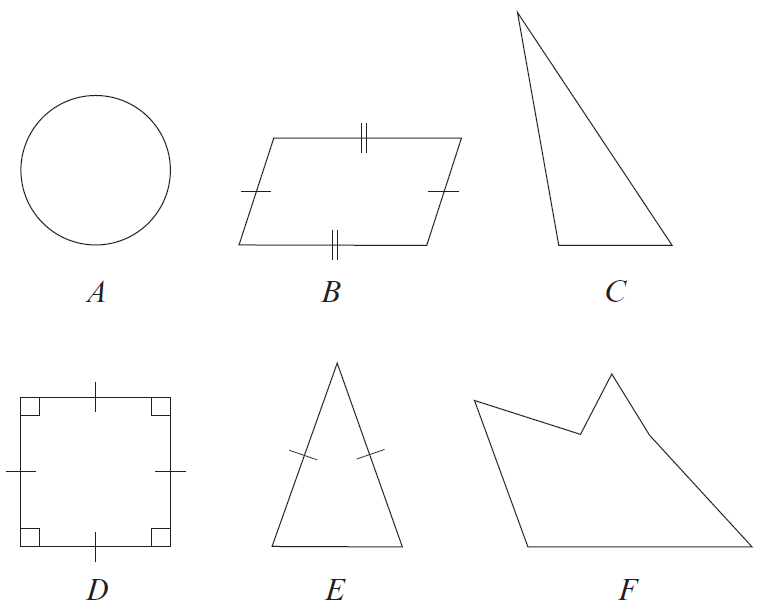
\includegraphics[width=10cm]{pictures/kpl3_2_teht7}
\end{center}

\item
Olkoot $S(x)$ avoin lause ''kuvio $x$ on symmetrinen
jonkin suoran suhteen'' ja $P(x)$ avoin lause ''kuvio $x$
on symmetrinen jonkin pisteen suhteen''. Perusjoukon
muodostavat oheiset kuviot. Ratkaise avoin lause.
\begin{enumerate}[a)]
\item $S(x)$,
\item $P(x)$,
\item $\lnot (S(x) \lor P(x))$,
\item $S(x) \lequiv P(x)$.
\end{enumerate}




\item
Arvotaan kaksi lukua, joista molemmat voivat olla 1, 2 tai 3. Arvonnan tuloksena saadaan lukupari $(x, y)$, missä $x$ on ensimmäisen arvonnan tulos ja $y$ toisen arvonnan tulos. Olkoot avoimet lauseet $S(x, y)$: ''$x \le y$'' ja $T(x, y)$: ''tulo $xy$ on jaollinen luvulla 3''. Ratkaise avoin lause, kun perusjoukon muodostavat arvonnan tuloksena saatavat mahdolliset lukuparit
\[
(1, 1),\ (1, 2),\ (1, 3),\ (2, 1),\ (2, 2),\ (2, 3),\ (3, 1),\ (3, 2),\ (3, 3).
\]
\begin{enumerate}[a)]
\item $S(x, y)$,
\item $\lnot T(x, y)$,
\item $\lnot (S(x, y) \lor T(x, y))$,
\item $S(x, y) \to T(x, y)$.
\end{enumerate}

\item
Ratkaise reaalilukujen joukossa
\begin{enumerate}[a)]
\item epäyhtälö $x^2 \le 4$,
\item epäyhtälöpari
\[
\left\{
\begin{array}{rcl}
x^2 & \le & 4 \\
x & > & -1.
\end{array}\right.
\]
\end{enumerate}

\item
Ratkaise reaalilukujen joukossa epäyhtälö
\begin{enumerate}[a)]
\item $|x| > 5$,
\item $|x| \le 1$,
\item $|x - 4| > 5$,
\item $|2x - 6| \le 1$.
\end{enumerate}

\item Ratkaise avoin lause reaalilukujen joukossa. Ilmaise ratkaisujoukko myös välimerkintää käyttäen.
\begin{enumerate}[a)]
\item $(x^2 > 1) \lor (0 \le x \le 2)$,
\item $(x^2 > 1) \land (0 \le x \le 2)$,
\item $(x^2 > 1) \to (0 \le x \le 2)$.
\end{enumerate}

\item
Olkoot $P(x)$ avoin lause $(x < 10) \land (x^2 = 100)$ ja
$Q(x)$ avoin lause $(x \ge 10) \lequiv (x^2 = 100)$. Ratkaise avoin lause reaalilukujen joukossa.
\begin{enumerate}[a)]
\item $P(x)$,
\item $Q(x)$,
\item $P(x) \lor Q(x)$,
\item $P(x) \land Q(x)$.
\end{enumerate}


\end{enumerate}

\subsection*{Kotitehtäviä}

\begin{enumerate}

\item
Olkoon $T(x, y)$ avoin lause ''$x$ lähettää tekstiviestin
$y$:lle''. Suomenna lause.
\begin{enumerate}[a)]
\item $T(\textrm{Tiina}, \textrm{Elias})$,
\item $\lnot T(\textrm{Elias}, \textrm{Tiina}) \land T(\textrm{Elias}, \textrm{Vilma})$,
\item $T(x, x)$,
\item $T(y, \textrm{Rasmus}) \lequiv T(\textrm{Rasmus}, y)$.
\end{enumerate}

\item
Olkoot $E(x)$ avoin lause ''$x$ on eurooppalainen
pääkaupunki'' ja $S(x)$ avoin lause ''$x$ on suomalainen
kaupunki''. Ratkaise avoin lause, kun perusjoukko on
$\{\textrm{Helsinki}, \textrm{Rovaniemi}, \textrm{Praha}, \textrm{Milano}\}$.
\begin{enumerate}[a)]
\item $E(x)$,
\item $\lnot S(x)$,
\item $S(x) \land \lnot E(x)$,
\item $\lnot (E(x) \land S(x))$,
\item $E(x) \lequiv S(x)$.
\end{enumerate}

\item
Olkoon $R(x)$ avoin lause ''$x^2 - 100 > 0$''. Onko lause
a) $R(10)$ b) $R(-15)$ tosi?

\item
Olkoon $S(x, y)$ avoin lause ''$x^2 + y^2 = 5$''. Onko
lause a) $S(2, 3)$ b) $S(2, -1)$ c) $S(-\sqrt{5}, 0)$ d)
$S(-1, -1)$ tosi?

\item
Ratkaise avoin lause $9x^2 + 30x + 25 \le 0$, kun
määrittelyjoukko on a) reaalilukujen joukko b)
kokonaislukujen joukko.

\item
Olkoot perusjoukko $\{ 1, 2, 3, \ldots , 16\}$, $C(x)$
avoin lause ''luku 12 on jaollinen luvulla $x$'' ja $D(x)$ avoin lause ''luvun $x$ neliöjuuri on kokonaisluku''.
Ratkaise avoin lause.
\begin{enumerate}[a)]
\item $C(x)$,
\item $D(x)$,
\item $\lnot C(x) \land D(x)$,
\item $C(x) \lequiv D(x)$.
\end{enumerate}

\item
Arvotaan kolme lukua, joista jokainen voi olla 1 tai
2. Arvonnan tuloksena saadaan lukukolmikko $(x, y, z)$, missä $x$ on ensimmäisen arvonnan tulos, $y$ toisen arvonnan tulos ja $z$ kolmannen arvonnan tulos. Olkoot
avoimet lauseet $S(x, y, z)$: ''$x + y + z \ge 5$'', $T(x,
y, z)$: ''tulo $xyz$ on pariton'' ja $U(x, y, z)$: “summa
$x + y + z$ on jaollinen luvulla 3''. Ratkaise avoin
lause, kun perusjoukon muodostavat arvonnan tuloksena
saatavat mahdolliset lukukolmikot
\[
(1, 1, 1),\ (1, 1, 2),\ (1, 2, 1),\ (1, 2, 2),\ (2, 1, 1),\ (2, 1, 2),\ (2, 2, 1),\ (2, 2, 2).
\]
\begin{enumerate}[a)]
\item $S(x, y, z)$,
\item $T(x, y, z)$,
\item $U(x, y, z)$,
\item $S(x, y, z) \land T(x, y, z)$,
\item $S(x, y, z) \lor \lnot U(x, y, z)$,
\item $\lnot (S(x, y, z) \lor T(x, y, z) \lor U(x, y, z))$,
\item $S(x, y, z) \land (T(x, y, z) \lequiv U(x, y, z))$.
\end{enumerate}

\item
Ratkaise reaalilukujen joukossa.
\begin{enumerate}[a)]
\item $x^2 = 1$ tai $x(x + 5)(x - 1) = 0$
\item $x^2 = 1$ ja $x(x + 5)(x - 1) = 0$
\end{enumerate}

\item
Ratkaise reaalilukujen joukossa
\begin{enumerate}[a)]
\item epäyhtälö $x^2 - 11x + 30 > 0$,
\item epäyhtälöpari
\[
\left\{
\begin{array}{rcl}
x^2 - 11x + 30 & > & 0 \\
2x & > & -6 - x.
\end{array}\right.
\]
\end{enumerate}

\item Ratkaise avoin lause reaalilukujen joukossa. Ilmaise ratkaisujoukko myös välimerkintää käyttäen.
\begin{enumerate}[a)]
\item $(-4 < x) \lor (x < 8)$,
\item $(-4 < x) \land (x < 8)$,
\item $((-4 < x) \land (x < 8)) \land (-5 \le x \le -3)$,
\item $(-4 < x) \lequiv (-5 \le x \le -3)$.
\end{enumerate}

\item
Olkoot $A(x)$ avoin lause $(x \ge 0) \to (x \ge 20)$
ja $B(x)$ avoin lause $\lnot ((x \le 0) \lor (x \ge 20))$. Ratkaise avoin lause reaalilukujen joukossa.
\begin{enumerate}[a)]
\item $A(x)$,
\item $B(x)$,
\item $A(x) \lor B(x)$.
\end{enumerate}

\end{enumerate}



\newpage

\section{Kvanttorit}
\termi{kvanttori}{Kvanttorien} avulla voidaan ilmaista täsmällisesti yleisluontoisia väitteitä, kuten tämän kirjan ensimmäisessä luvussa annettu esimerkki: ''kaikki joutsenet ovat valkoisia''. Tavoitteena on muodostaa loogisesti päteviä päätelmiä, jotka koskevat esimerkiksi jonkin joukon kaikkia alkioita.

\subsection*{Tutkimustehtävä}
Ovatko seuraavat väitteet tosia?
\begin{enumerate}
\item Kaikki koulumme opiskelijat opiskelevat englantia.
\item Kaikki koulumme opiskelijat opiskelevat pitkää matematiikkaa.
\item Koulussamme on opiskelija, joka harrastaa kilpaurheilua.
\item Koulussamme on opiskelija, joka on tämän vuoden Miss Suomi.
\item Kirjoita kohtien 1 ja 3 väitteiden negaatiot kahdella eri tavalla. 
\end{enumerate}

Predikaattilogiikassa määritellään kaksi kvanttoria, $\exists$ ja $\forall$. Näistä ensimmäistä kutsutaan \termi{eksistenssikvanttori}{eksistenssikvanttoriksi} eli \termi{olemassaolokvanttori}{olemassaolokvanttoriksi}. Lause
\[
\exists x\, P(x)
\]
tarkoittaa, että perusjoukossa $X$ on ainakin yksi alkio, jolla on ominaisuus $P$. Toisin sanoen joukko $P$ ei ole tyhjä joukko. Lause luetaan: ''On olemassa $x$ siten, että $P(x)$''.

Kvanttoria $\forall$ kutsutaan \termi{universaalikvanttori}{universaalikvanttoriksi} eli \termi{kaikkikvanttori}{kaikkikvanttoriksi}. Lause
\[
\forall x\, P(x)
\]
tarkoittaa, että ominaisuus $P$ on kaikilla perusjoukon $X$ alkioilla. Lause luetaan: ''Kaikille $x$ pätee $P(x)$''.

Kvanttorien avulla voidaan esittää matemaattisia väittämiä hyvin tiiviissä ja täsmällisessä muodossa. Tästä on hyötyä etenkin matemaattisessa logiikassa, jossa tutkimuskohteena ovat matemaattiset teoriat, tulokset ja todistukset. 

\begin{esimerkki}
%{\bf Esimerkki 1.}
Liikuntailtapäivässä koulun opiskelijat harrastavat eri talviurheilulajeja. Olkoot perusjoukko koulun opiskelijat ja avoimet lauseet $H(x)$: ''opiskelija $x$
 hiihtää'' ja $L(x)$: ''opiskelija $x$ laskettelee lumilaudalla''.

Kirjoita suomen kielellä lauseet a) $\forall x H(x)$,  b)  $\exists x L(x)$. Milloin lause on tosi? Milloin lause on epätosi?

{\bf Ratkaisu:} a) Lause tarkoittaa, että kaikki koulun opiskelijat hiihtävät. Lause on tosi silloin, kun
kaikki opiskelijat hiihtävät. Lause on epätosi silloin, kun on ainakin yksi opiskelija, joka ei 
hiihdä.  

b) Lause tarkoittaa, että joku koulun opiskelija laskettelee lumilaudalla. Lause on tosi
silloin, kun ainakin yksi opiskelija laskettelee lumilaudalla. Lause on epätosi silloin, kun 
kukaan koulun opiskelijoista ei laskettele lumilaudalla. 
\end{esimerkki}

\begin{esimerkki}
%{\bf Esimerkki 2.}
Olkoot perusjoukko reaalilukujen joukko $\R$ ja avoimet lauseet  $P(x)$: ''$x^2 > 0$''  sekä  
$Q(x)$: ''$x^2\le  0$''. Suomenna lauseet  a) $\forall x P(x)$,   b) $\exists x Q(x)$. Ovatko lauseet tosia?

{\bf Ratkaisu:}	a) Lause tarkoittaa, että kaikkien reaalilukujen neliöt ovat positiivisia. Lause on epätosi, sillä luvun $0$ neliö ei ole positiivinen: $0^2=0$.

Lauseen epätodeksi osoittamiseen siis riittää, että on olemassa yksikin alkio (niin sanottu \termi{vastaesimerkki}{vastaesimerkki}), jolle avoin lause $P(x)$ on epätosi.

b)  Lause tarkoittaa, että on olemassa reaaliluku, jonka neliö on pienempi tai 
yhtä suuri kuin nolla. Lause on tosi, sillä $0^2 = 0$.

Lauseen todeksi osoittamiseen siis riittää, että on olemassa yksikin alkio, jolle avoin lause $Q(x)$ on tosi.

{\bf Vastaus:}	
a) Kaikkien reaalilukujen neliöt ovat positiivisia. Lause on epätosi.

b) On olemassa reaaliluku, jonka neliö on pienempi tai yhtä suuri kuin nolla. Lause on tosi. 
\end{esimerkki}

\begin{esimerkki}
%{\bf Esimerkki 3.}
Onko lause tosi? Perustele.
\begin{enumerate}[a)]
\item $\exists x\in \Z(4x - 3 = 0)$
\item $\forall x\in \R(-x^2 + x \le 2)$
\end{enumerate}

{\bf Ratkaisu:}

a) Yhtälön $4x - 3 = 0$ ratkaisu on $x = \frac{3}{4}$. Koska luku $\frac{3}{4}$ ei ole kokonaisluku, lause $\exists x\in \Z(4x - 3 = 0)$ on epätosi.

b) Epäyhtälö $-x^2+x \le 2$ on yhtäpitävä epäyhtälön $0 \le x^2 - x + 2$ kanssa. Tutkitaan polynomifunktion $x^2 - x + 2$ merkkiä. Ratkaistaan funktion $x^2 - x + 2$ nollakohdat toisen asteen yhtälön ratkaisukaavalla.
\[
x^2 - x + 2 = 0
\]
\[
x=\frac{-(-1) \pm \sqrt{(-1)^2 -4\cdot 1 \cdot 2}}{2 \cdot 1}=\frac{1 \pm \sqrt{-7}}{2}
\]
Funktiolla ei ole nollakohtia, koska diskriminantti $-7$ on negatiivinen. 

\bigskip

\begin{center}
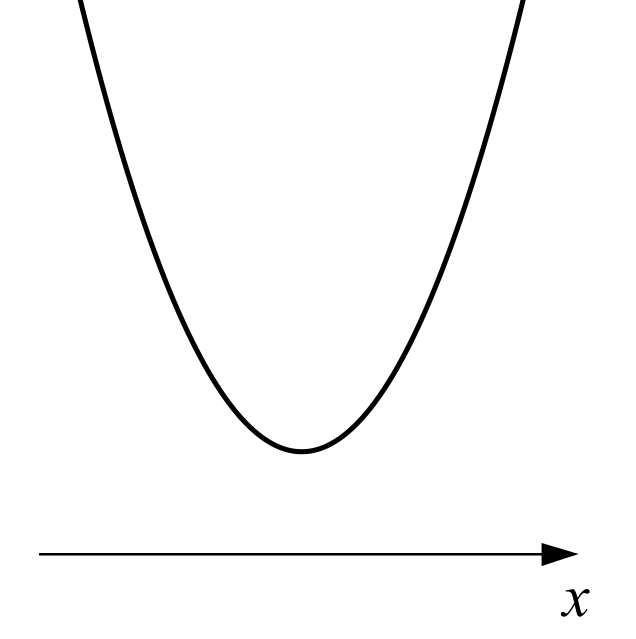
\includegraphics[width=4.5cm]{pictures/kpl3_3_paraabeli}
\end{center}

Koska funktion $x^2 - x + 2$ kuvaaja on ylöspäin aukeava paraabeli, funktio saa vain positiivisia arvoja. Siten epäyhtälö $0 \le x^2 - x + 2$ toteutuu kaikilla muuttujan $x$ arvoilla. Lause $\forall x\in \R(-x^2 + x \le 2)$ on siis tosi.

{\bf Vastaus:} a) Lause on epätosi. b) Lause on tosi.
\end{esimerkki}

\begin{esimerkki}
%{\bf Esimerkki 4.}
Suomenna lause
\begin{enumerate}[a)]
\item $\forall x\in \Z\exists y\in \Z (x+y=0)$
\item $\exists y\in \R\forall x\in \R (x+y =x)$.
\end{enumerate}
Onko lause tosi?

{\bf Ratkaisu:}

a) Lause tarkoittaa, että jokaista kokonaislukua $x$ kohden on
olemassa sellainen kokonaisluku $y$, että lukujen summa on nolla.

Lause on tosi, sillä jokaisella kokonaisluvulla on vastaluku,
joka on kokonaisluku. Luvun ja sen vastaluvun summa on nolla.

b) Lause tarkoittaa, että on olemassa sellainen reaaliluku $y$,
että sen ja minkä tahansa reaaliluvun $x$ summa on aina yhtä
suuri kuin $x$.

Lause on tosi, sillä nolla on tällainen reaaliluku.

{\bf Vastaus:} a) Jokaista kokonaislukua $x$ kohden on olemassa
sellainen kokonaisluku $y$, että lukujen summa on nolla. Lause on
tosi.

b) On olemassa sellainen reaaliluku $y$, että sen ja minkä
tahansa reaaliluvun $x$ summa on aina $x$. Lause on tosi.
\end{esimerkki}

\subsection*{Kvanttorien negaatiot} Tutkitaan lausetta ''kaikki joutsenet ovat valkoisia''. Lause voidaan formalisoida kaikkikvanttorin avulla $\forall x V(x)$, missä perusjoukkona on joutsenten joukko $J$ ja $V(x)$ on lause ''$x$ on valkoinen''. Tämä lause osoittautui epätodeksi, kun Australiasta löydettiin mustia joutsenia. Lauseen $\forall x V(x)$ negaatio $\lnot \forall x V(x)$ voidaan kirjoittaa $\exists x \lnot V(x)$ ja suomentaa ''on olemassa (ainakin yksi) joutsen, joka ei ole valkoinen''. Vastaavasti lauseen $\exists x V(x)$ negaatio $\lnot \exists x V(x)$ eli ''ei ole olemassa valkoista joutsenta'' voidaan lausua ekvivalentissa muodossa $\forall x \lnot V(x)$. Tämä lause voidaan hieman kömpelösti kielentää ''kaikki joutsenet ovat ei-valkoisia''.

%---
%{\bf Teorialaatikko [Kvanttorien negaatiot].} 
%\fbox{
%\begin{minipage}{12cm}
\laatikko{
{\bf Kvanttorien negaatiot.}
%\medskip
Olkoon $P(x)$ avoin lause. Tällöin
\begin{itemize}
\item 
lause $\lnot \forall xP(x)$ on loogisesti ekvivalentti lauseen $\exists x\lnot P(x)$ kanssa, ja
\item
 lause $\lnot \exists xP(x)$ on loogisesti ekvivalentti lauseen $\forall x\lnot P(x)$ kanssa.
\end{itemize}
%\end{minipage}
}
%---

Saatu kvanttorien negaatioita koskeva tulos muotoillaan joskus myös toisella tavalla. Koska lause $\lnot \forall x V(x)$ on loogisesti ekvivalentti lauseen $\exists x\lnot V(x)$ kanssa, voidaan päätellä, että lause $\forall x V(x)$ on loogisesti ekvivalentti lauseen $\lnot \exists x\lnot V(x)$ kanssa. Vastaava päättely voidaan tehdä myös eksistenssikvanttorin tapauksessa.


\begin{esimerkki}
%{\bf Esimerkki 5.}
Muodosta lauseen
\begin{enumerate}[a)]
\item $\forall x \in \R(-x^2 \le 0)$
\item $\exists x\in \N(2x-3>0)$
\end{enumerate}
negaatio. Onko negaatio tosi?

{\bf Ratkaisu:}

a) Lauseen $\forall x \in \R(-x^2 \le 0)$ negaatio on loogisesti ekvivalentti lauseen $\exists x\in \R (-x^2 > 0)$ kanssa.

Lause $\exists x\in \R (-x^2> 0)$ on epätosi, sillä tunnetusti $x^2$ on aina suurempi tai yhtä suuri kuin nolla. Siten $-x^2$ on aina pienempi tai yhtä suuri kuin nolla.

b) Lauseen $\exists x\in \N(2x-3>0)$ negaatio on loogisesti ekvivalentti lauseen $\forall x\in \N(2x-3 \le 0)$ kanssa.

Lause $\forall x\in \N(2x-3 \le 0)$ on epätosi, sillä esimerkiksi tapauksessa $x=5$ saadaan lausekkeen $2x - 3$ arvoksi $2\cdot 5 -3 = 7$, joka ei ole pienempi tai yhtä suuri kuin nolla.

{\bf Vastaus:} a) $\exists x\in \R (-x^2 > 0)$. Negaatio on epätosi. 

b) $\forall x\in \N(2x-3 \le 0)$. Negaatio on epätosi.
\end{esimerkki}


%\newpage

%\section*{Tehtäviä}

\Harjoitustehtavat

\begin{enumerate}

\item Olkoon perusjoukko kaikki koulun opiskelijat. Olkoon lause
$T(x)$: ''opiskelija $x$ on täysi-ikäinen''. Suomenna lause.
\begin{enumerate}[a)]
\item $\forall x T(x)$
\item $\exists x T(x)$
\item $\exists x \lnot T(x)$
\item $\forall x \lnot T(x)$
\end{enumerate}

\item Suomenna lause. Onko lause tosi? Perustele.
\begin{enumerate}[a)]
\item $\forall x\in\R (|x| > 0)$
\item $\forall x\in\R (|x| \ge 0)$
\item $\exists x\in\N (x^2 < 2)$
\item $\exists x\in\N (x^2 = 2)$
\end{enumerate}

\item
Formalisoi lause. Onko lause tosi? Perustele.
\begin{enumerate}[a)]
\item Jokainen kokonaisluku on joko positiivinen tai
negatiivinen.
\item On olemassa sellainen kokonaisluku, jonka neliöjuuri on
yhtä suuri kuin luku itse.
\item Minkään kokonaisluvun neliö ei ole $7$.
\end{enumerate}

\item Osoita, että yhtälö $\sqrt{x^2} = x$ ei pidä paikkaansa
kaikilla reaaliluvuilla.

\item Jalkapallojoukkue on lähdössä turnausmatkalle. Olkoon
$P(x, y)$ avoin lause ''pelaajalla $x$ on pelaajan $y$
puhelinnumero''. Suomenna lause.
\begin{enumerate}[a)]
\item $\forall x \exists y P(x, y)$
\item $\exists x \forall y P(x, y)$
\item $\exists y \forall x P(x, y)$
\end{enumerate}

\item
Formalisoi lause. Onko lause tosi?
\begin{enumerate}[a)]
\item Positiivisten kokonaislukujen joukossa on pienin alkio.
\item Negatiivisten kokonaislukujen joukossa on pienin alkio.
\end{enumerate}

\item Onko lause tosi? Perustele.
\begin{enumerate}[a)]
\item $\forall x\in \R\exists y\in \R (xy=1)$
\item $\exists y\in \R\forall x\in \R (xy =x)$
\end{enumerate}

\item Olkoon $M(x)$: ''$x$ on matemaatikko''. Formalisoi lause.

\begin{enumerate}[a)]
\item Kaikki eivät ole matemaatikkoja.
\item Joku ei ole matemaatikko.
\item Ei ole olemassa matemaatikkoa.
\item Kukaan ei ole matemaatikko.
\end{enumerate}

\item
Muodosta lauseen negaatio.
\begin{enumerate}[a)]
\item $\forall x\in \Z (x < 12)$
\item $\exists x\in \Z (x^2 = 12)$
\item $\exists x\in \N ((x^2=9) \land (x<5))$
\item $\forall x\in \N ((x=0)\lor (x\ge 1))$
\end{enumerate}

\item Osoita, että lause $\exists a, b, c \in \Z_{+} (a^2 + b^2 =
c^2)$ on tosi.

\item * % (Lisämateriaalia) 
Olkoot $M(x)$: ''$x$ on matemaatikko'' ja
$I(x)$: ''$x$ on iloinen''. Formalisoi lause.
\begin{enumerate}[a)]
\item Kaikki ovat iloisia matemaatikkoja.
\item Matemaatikot ovat iloisia.
\item Kukaan matemaatikko ei ole iloinen.
\item Kaikki matemaatikot eivät ole iloisia.
\end{enumerate}

\item * %(Lisämateriaalia)
Olkoot $K(x)$: ''$x$ on kampaaja'' ja
$T(x, y)$: ''$x$ tekee $y$:lle kampauksen''. Formalisoi lause.
\begin{enumerate}[a)]
\item Kukaan kampaaja ei tee kampausta itselleen.
\item Joku kampaaja tekee kampauksen niille kampaajille,
jotka eivät tee kampausta itselleen.
\end{enumerate}

\end{enumerate}

\subsection*{Kotitehtäviä}

\begin{enumerate}

\item Olkoon perusjoukko $xy$-tason suorien joukko. Olkoot
lauseet $N(x)$: ''suora on nouseva'' ja $L(x)$: ''suora on laskeva''.
Suomenna lause. Onko lause tosi?
\begin{enumerate}[a)]
\item $\exists x L(x)$
\item $\forall x (N(x) \lor L(x))$
\item $\exists x (\lnot N(x) \land \lnot L(x))$
\item $\forall x \lnot N(x)$
\end{enumerate}

\item Onko lause tosi? Perustele.
\begin{enumerate}[a)]
\item $\forall x\in\R (x^2 \ge 0)$
\item $\exists x\in\N (x^2 = -9)$
\item $\forall x\in\R ((x-1)(x-3) \ge 0)$
\item $\exists x\in\Z (-x^2 - 2 \le 0)$
\end{enumerate}

\item Onko lause tosi? Perustele.
\begin{enumerate}[a)]
\item $\exists x\in \R (x^2 - 3x + 3 = 0)$
\item $\forall x\in \R (x^2 - 3x + 3 \ge 0)$
\end{enumerate}

\item
\begin{enumerate}[a)]
\item Osoita, että yhtälö $\sqrt{xy} = \sqrt{x}\sqrt{y}$ ei
pidä paikkaansa kaikilla reaaliluvuilla $x$ ja $y$.
\item Osoita, että on olemassa sellaiset reaaliluvut $x$ ja
$y$, että yhtälö $\sqrt{xy} = \sqrt{x}\sqrt{y}$ pitää paikkansa.
\item Millä ehdolla yhtälö $\sqrt{xy} = \sqrt{x}\sqrt{y}$
pitää yleisesti paikkansa?
\end{enumerate}

\item Olkoon $S(x, y)$: ''$x$ on suorittanut kurssin $y$''.
Formalisoi lause.
\begin{enumerate}[a)]
\item Joku on suorittanut kaikki kurssit.
\item Jokainen on suorittanut ainakin yhden kurssin.
\item Kukaan ei ole suorittanut kaikkia kursseja.
\item On olemassa kurssi, jota kukaan ei ole suorittanut.
\end{enumerate}

\item Onko lause tosi? Perustele.
\begin{enumerate}[a)]
\item $\forall x\in \Z_{+} \exists y\in \Z_{+} (x = \sqrt{y})
$
\item $\exists y\in \R \forall x\in \R (x^2 - 4 > y)$
\end{enumerate}

\item Ilmaise suomen kielellä lauseen negaatio kahdella eri
tavalla soveltamalla kvanttorien negaatioiden loogisesti
ekvivalentteja muotoja.
\begin{enumerate}[a)]
\item Jokainen opiskelija saa tästä kurssista arvosanan 10.
\item On olemassa opiskelija, joka saa tästä kurssista
arvosanan 10.
\end{enumerate}

\item Kirjoita lause toisin.
\begin{enumerate}[a)]
\item $\lnot \forall x \lnot P(x)$
\item $\lnot \exists x (P(x) \lor Q(x))$
\end{enumerate}

\item
Muodosta lauseen negaatio. Onko negaatio tosi?
\begin{enumerate}[a)]
\item $\forall x\in ]1, \infty [ (\sqrt{x} < x)$
\item $\exists x\in \Q (x^3 = 5)$
\item $\forall n \in \Z \exists m \in \Z ((n = 2m) \lor (n =
2m+1))$
\end{enumerate}

\item Funktiota $f\colon X\to Y$ voidaan ajatella kahden
muuttujan avoimena lauseena $P(x, y)$: ''$f(x) = y$'', missä
$x$ kuuluu määrittelyjoukkoon $X$ ja $y$ maalijoukkoon $Y$.
Funktiolta edellytetään lisäksi, että
\begin{itemize}
\item $\forall x \exists y P(x, y)$, ja
\item $\lnot (\exists x \exists y \exists z (P(x, y) \land P(x, z)
\land (y \neq z)))$.
\end{itemize}
Tulkitse sanallisesti tai kuvaa käyttäen, mitä tämä määritelmä
tarkoittaa.

\item * %(Lisämateriaalia)
 Olkoot $S(x, y)$: ''$x$ on suorittanut
kurssin $y$'' ja $L(x)$: ''$x$ on lukiolainen''. Formalisoi lause.
\begin{enumerate}[a)]
\item Joku lukiolainen on suorittanut kaikki kurssit.
\item Kukaan lukiolainen ei ole suorittanut kaikkia kursseja.
\end{enumerate}

\item * %(Lisämateriaalia)
Olkoot $S(x, y)$: ''$x$ on suorittanut
kurssin $y$'', $L(x)$: ''$x$ on lukiolainen'' ja $M(y)$: ''$y$ on
pitkän matematiikan kurssi''. Formalisoi lause.
\begin{enumerate}[a)]
\item Joku lukiolainen ei ole suorittanut yhtään pitkän
matematiikan kurssia.
\item Joku lukiolainen on suorittanut pitkän matematiikan
kurssin.
\item Jokaisella lukiolaisella on pitkän matematiikan kurssi
suoritettuna.
\item On olemassa pitkän matematiikan kurssi, jota kukaan
lukiolainen ei ole suorittanut.
\end{enumerate}

\item * %(Lisämateriaalia)
Määritä kaikki funktiot $f\colon X\to Y$,
kun $X=\{a, b, c\}$ ja $Y=\{1, 2\}$.

\item * %(Lisämateriaalia)
Määritä kaikki funktiot $f\colon X\to Y$,
kun $X=\emptyset$ ja $Y\neq \emptyset$.

\item * %(Lisämateriaalia)
Määritä kaikki funktiot $f\colon X\to Y$,
kun $X\neq \emptyset$ ja $Y= \emptyset$.

%%%%%%%%%%%%%%%%%%%%%%%%%%%%%%%FIX ME, linkki toimimaton  %%%%%%%
\item * %(Lisämateriaalia)
Tutustu logiikkapohjaiseen Prolog-ohjelmointikieleen\\
\href{http://www.cs.helsinki.fi/u/wikla/OKP/OppaatK07/prolog.html}
{{\tt http://www.cs.helsinki.fi/u/wikla/OKP/OppaatK07/prolog.html}}

Lataa koneellesi Prolog-tulkki \href{http://www.gprolog.org/}
{{\tt http://www.gprolog.org/}}
ja kokeile Prolog-ohjelmointia.

\end{enumerate}
